% Options for packages loaded elsewhere
\PassOptionsToPackage{unicode}{hyperref}
\PassOptionsToPackage{hyphens}{url}
%
\documentclass[
]{article}
\usepackage{amsmath,amssymb}
\usepackage{lmodern}
\usepackage{ifxetex,ifluatex}
\ifnum 0\ifxetex 1\fi\ifluatex 1\fi=0 % if pdftex
  \usepackage[T1]{fontenc}
  \usepackage[utf8]{inputenc}
  \usepackage{textcomp} % provide euro and other symbols
\else % if luatex or xetex
  \usepackage{unicode-math}
  \defaultfontfeatures{Scale=MatchLowercase}
  \defaultfontfeatures[\rmfamily]{Ligatures=TeX,Scale=1}
\fi
% Use upquote if available, for straight quotes in verbatim environments
\IfFileExists{upquote.sty}{\usepackage{upquote}}{}
\IfFileExists{microtype.sty}{% use microtype if available
  \usepackage[]{microtype}
  \UseMicrotypeSet[protrusion]{basicmath} % disable protrusion for tt fonts
}{}
\makeatletter
\@ifundefined{KOMAClassName}{% if non-KOMA class
  \IfFileExists{parskip.sty}{%
    \usepackage{parskip}
  }{% else
    \setlength{\parindent}{0pt}
    \setlength{\parskip}{6pt plus 2pt minus 1pt}}
}{% if KOMA class
  \KOMAoptions{parskip=half}}
\makeatother
\usepackage{xcolor}
\IfFileExists{xurl.sty}{\usepackage{xurl}}{} % add URL line breaks if available
\IfFileExists{bookmark.sty}{\usepackage{bookmark}}{\usepackage{hyperref}}
\hypersetup{
  pdftitle={A summary of Postesia palmaeformis studies to inform stewardship},
  pdfauthor={Karina J. Nielsen},
  hidelinks,
  pdfcreator={LaTeX via pandoc}}
\urlstyle{same} % disable monospaced font for URLs
\usepackage[margin=1in]{geometry}
\usepackage{longtable,booktabs,array}
\usepackage{calc} % for calculating minipage widths
% Correct order of tables after \paragraph or \subparagraph
\usepackage{etoolbox}
\makeatletter
\patchcmd\longtable{\par}{\if@noskipsec\mbox{}\fi\par}{}{}
\makeatother
% Allow footnotes in longtable head/foot
\IfFileExists{footnotehyper.sty}{\usepackage{footnotehyper}}{\usepackage{footnote}}
\makesavenoteenv{longtable}
\usepackage{graphicx}
\makeatletter
\def\maxwidth{\ifdim\Gin@nat@width>\linewidth\linewidth\else\Gin@nat@width\fi}
\def\maxheight{\ifdim\Gin@nat@height>\textheight\textheight\else\Gin@nat@height\fi}
\makeatother
% Scale images if necessary, so that they will not overflow the page
% margins by default, and it is still possible to overwrite the defaults
% using explicit options in \includegraphics[width, height, ...]{}
\setkeys{Gin}{width=\maxwidth,height=\maxheight,keepaspectratio}
% Set default figure placement to htbp
\makeatletter
\def\fps@figure{htbp}
\makeatother
\setlength{\emergencystretch}{3em} % prevent overfull lines
\providecommand{\tightlist}{%
  \setlength{\itemsep}{0pt}\setlength{\parskip}{0pt}}
\setcounter{secnumdepth}{5}
\ifluatex
  \usepackage{selnolig}  % disable illegal ligatures
\fi

\title{A summary of \emph{Postesia palmaeformis} studies to inform stewardship}
\author{Karina J. Nielsen}
\date{Last compiled on 14 June 2021}

\begin{document}
\maketitle

{
\setcounter{tocdepth}{2}
\tableofcontents
}
\hypertarget{introduction}{%
\section{Introduction}\label{introduction}}

This document presents a summary of published research on the ecology of intertidal sea palm kelp \emph{Postelsia palmaeformis} (hereafter \emph{Postelsia}) together with new analyses of unpublished data collected by \href{http://www.faralloninstitute.org/sarah-ann}{Sarah Ann Thompson}, Heather Knoll, \href{https://vesr.nrs.ucsb.edu/about/people/dr-carol-blanchette}{Carol Blanchette}, and \href{https://karinanielsen.io/}{Karina Nielsen} as part of a \href{https://caseagrant.ucsd.edu/sites/default/files/RCZ-200-Nielsen.pdf}{CA Sea Grant funded research project} to KN and CB. The focus of that project was to examine the effects of artisanal commercial harvesting in California on \emph{Postelsia}.

The California Fish and Game Commission is receiving requests to limit commercial seaweed harvesting in response to the collapse of \emph{Nereocystis leutkeana} bull kelp forests \href{https://www.nature.com/articles/s42003-021-01827-6}{(McPherson et al.~2021)} and concerns that there may be a concurrent decline of \emph{Postelsia} populations in some locations. In addition a \href{https://static1.squarespace.com/static/5db26a9129f30174496b208b/t/608106c52665aa1e0bb1ab43/1619068616608/DRAFT+Tribal+Proposal+for+Amending+Commercial+Kelp+\%26+Seaweed+Rules-Updated+4.21.2021-PDF.pdf}{proposal} developed by the \href{https://sinkyone.org/}{Intertribal Sinkyone Wilderness Council} for a moratorium on commercial harvesting of these two species has also been submitted for consideration.\\
This summary is presented as an open science project to support stewardship decisions and provide stakeholders with available scientific information on \emph{Postelsia}. The data and code used to create this document and conduct analyses of unpublished data are available in \href{https://github.com/phyllospadix/postelsia}{this public repository}. The new analyses of unpublished data presented here have not been peer-reviewed.

\begin{quote}
The bottom line: a precautionary approach to the stewardship of \emph{Postelsia palmaeformis} is warranted.
\end{quote}

\newpage

\hypertarget{biology-and-ecology}{%
\section{Biology and ecology}\label{biology-and-ecology}}

The \href{https://marine.ucsc.edu/target/target-species-postelsia.html}{sea palm \emph{Postelsia palmaeformis}} is an intertidal kelp (a brown macroalga in the Order Laminariales). It is only found on the west coast of North America. It grows a robust holdfast to attach to the rocks or mussels or barnacles where it settles (Figure @ref(fig:post-anat)). It has a hollow tubular stem-like stipe topped with a mop-like profusion of ridged blades (or fronds).

\begin{figure}

\includegraphics[width=0.3\linewidth]{https://web.archive.org/web/20071006173831im_/http://www.mbari.org/staff/conn/botany/browns/saraho/morphp} \hfill{}

\caption{Anatomy of *Postelsia* (illustration by Sarah Oehm).}(\#fig:post-anat)
\end{figure}

\emph{Postelsia} is an annual species with a heteromorphic life history (similar to ferns) alternating between two stages: 1) a microscopic, filamentous gametophyte and 2) a macroscopic sporophyte resembling a miniature palm tree.

\emph{Postelsia's} annual life history begins with the germination of haploid zoospores shed from sori (dark stripes where spores form) that develop on the fronds of mature thalli (or ``plants'') (Figure @ref(fig:post-cycle)). These grow into the microscopic male and female gametophytes. Sporophytes develop from the fusion of haploid gametes when sperm from a male gametophyte fertilizes an egg on a female gametophyte. The young spororphytes become visible on the shore in clusters of small plants \href{https://bodegahead.blogspot.com/search/label/postelsia}{in late winter}. They grow rapidly and develop sori on their fronds in June, but timing varies with latitude, harvesting, and differences in environmental conditions among years (Thompson et al.~2010, Nielsen et al.~unpublished data).

\begin{figure}

\includegraphics[width=0.6\linewidth]{https://web.archive.org/web/20070714142300im_/http://www.mbari.org/staff/conn/botany/browns/saraho/lifeani} \hfill{}

\caption{Life history cycle of *Postelsia* (animated illustration by Sarah Oehm).}(\#fig:post-cycle)
\end{figure}

During summer and fall when sea palms are reproductive, spores are released during low tide dribble down the grooved fronds. They usually do not disperse further than about 1.5 meters from the parent plants (Paine et al.~2017). When the sporophytes become reproductive, they stop investing in growth or re-growth of fronds (Nielsen et al.~2010). They do not regrow from the stipe if it is cut or breaks off. The active growth region (meristem) is located at the base of the fronds above the top of the stipe. The mature sporophytes begin obvious senesence in the late fall. Most are eventually torn off the rocks by winter storms (Dayton 1973, Paine 1979, Blanchette 1996). \emph{Postelsia} are highly productive and their dislodged thalli help fuel wrack-dependent food webs on sandy beaches throughout the growing season (Leigh et al.~1987, Leibowitz et al.~2016).

Sea palm populations are patchily distributed in the intertidal zone of very wave-exposed rocky shores. The discrete populations form a sheltering canopy habitat for smaller organisms including snails and limpets and a variety of seaweeds. Black oystercatchers and other shorebirds forage for these smaller invertebrates on wave exposed shores where sea palm populations occur.

\emph{Postelsia} is physiologically limited to wave exposed, mid-high intertidal zone (Nielsen et al.~2006). However, it's patchy population structure and meta-population dynamics are mediated by wave-driven disturbances (Dayton 1973, Paine 1979, Blanchette 1996). It forms dynamic, usually persistent local meta-populations, due to its annual, disturbance-mediated life history and the very short dispersal distance of its zoospores.

\newpage

\hypertarget{human-use-and-regulations-for-collecting-and-harvesting-postelsia}{%
\section{\texorpdfstring{Human use and regulations for collecting and harvesting \emph{Postelsia}}{Human use and regulations for collecting and harvesting Postelsia}}\label{human-use-and-regulations-for-collecting-and-harvesting-postelsia}}

\emph{Postelsia} and other seaweeds are traditional foods eaten by Indigenous Peoples \href{https://caseagrant.ucsd.edu/sites/default/files/39-Rocha-Final.pdf}{(Tolowa Dee-ni' Nation, et al.~2017)}. Edible seaweeds, including \emph{Postelsia}, are also an increasingly popular commercialized food product. The harvest of edible seaweeds in California has increased over the last two decades (Figure @ref(fig:post-harvest)). Commercial seaweed harvesting is not permitted in Oregon, Washington, and British Columbia.

\begin{figure}

\includegraphics[width=0.7\linewidth]{https://wildlife.ca.gov/portals/0/Images/marine/Kelp/EdibleHarvestData_12-14-20} \hfill{}

\caption{Commercial edible algae harvest logbook data, 1997-2019, [CDFW](https://wildlife.ca.gov/Conservation/Marine/Kelp/Commercial-Harvest)).}(\#fig:post-harvest)
\end{figure}

In California, \href{https://wildlife.ca.gov/Conservation/Marine/Kelp/Recreational-Harvest}{recreational harvest} of \emph{Postelsia} is prohibited, \href{https://wildlife.ca.gov/Licensing/Scientific-Collecting}{scientific collections} require a special authorization, and non-mechanized \href{https://wildlife.ca.gov/Conservation/Marine/Kelp/Commercial-Harvest}{commercial harvest} is allowed with the purchase of a commercial edible seaweed harvesting license. However, there is also no recognition in California regulations of Indigenous Peoples rights to traditional use of \emph{Postelsia} and other seaweeds. The number of commercial seaweed harvesting licenses, the amount of \emph{Postelsia} harvested, the method of its harvest, and the locations where harvesting is allowed, except for marine protected areas, are not regulated.

\newpage

\hypertarget{the-effect-of-frond-harvesting-on-juvenile-recruitment}{%
\section{The effect of frond harvesting on juvenile recruitment}\label{the-effect-of-frond-harvesting-on-juvenile-recruitment}}

In 2010 Thompson et al.~reported on two experiments done to evaluate the ecological consequences of commercial frond harvesting on \emph{Postelsia}. Commercial harvesters use a frond trimming method they claim is sustainable because the fronds regrow and allows multiple harvests per year. The research team from Thompson et al.~wondered if repeated harvests might reduce reproductive output and possibly reduce juvenile recruitment (population size in June) in the following year.

They did two studies to assess the effects of frond harvesting on \emph{Postelsia}. First they examining how frond regrowth and reproductive output at two sites, one in central and one in northern California, were impacted by frond harvesting at different times and different frequencies over the spring and summer growth season. In a second experiment they tracked 32 \emph{Postelsia} populations across four sites in northern California to see if frond harvesting would reduce juvenile recruitment in the following year. They repeated the harvest treatments and tracked the populations for three years. They also measured the sizes of individual thalli or ``plants'', determined the proportion of plants that were reproductive within each population, as well as the tidal elevation of each population.

Here we extend the analyses from the first two years (2007-2008) of these experiments, previously published by Thompson et al.~(2010), with new analyses and incorporating data collected in a subsequent year.

\newpage

\begin{quote}
The size of \emph{Postelsia} populations in August were a strong predictor of juvenile recruitment to the same locations the following year (Figure @ref(fig:pop-plot), Table 4.1). Frond harvesting, whether done once in the spring or twice over the spring and summer reduced the size of populations between 2007 and 2008, but not between 2008 and 2009. In 2008 recruitment was 38\% greater in populations not subjected to trimming and population sizes were reduced by 40-50\% when trimmed (Thompson et al.~(2010)). Juvenile recruitment (population size) was lower overall in June 2009 relative to June 2008.
\end{quote}

Table 4.1. Linear mixed model of \emph{Postelsia} recruitment.\\

~

Juvenile Recruitment

Predictors

Estimates

Conf. Int (95\%)

P-Value

Intercept

201.35

75.57~--~327.14

0.002

Adult pop. sz. prior yr.

1.02

0.88~--~1.17

\textless0.001

Harvested

-230.98

-372.20~--~-89.75

0.001

2009

-259.35

-413.00~--~-105.71

0.001

Harvested x 2009

312.58

125.98~--~499.17

0.001

Random Effects

σ2

28355.67

τ00 site\_code

1037.08

ICC

0.04

N site\_code

4

Observations

59

Marginal R2 / Conditional R2

0.779 / 0.786

The response variable is the abundance of juvenile \emph{Postelsia} plants in June for each population in the study. The explanatory variables are the abundance of adult parent plants in the prior August (augLag), and indicator variable for the frond harvest treatment (trim\_all, where 1 = fronds were harvested, 0 = fronds were left intact), the year (yr\_f, where year was either 2008 or 2009), and an interaction term between frond harvesting and year (trim\_all{[}1{]}*yr\_f{[}{[}2009{]}). The interaction term assesses if there was a different response to the frond harvesting treatment in 2009 compared to 2008. Sites were included as a random factor to account for the stratified randomization of trimming treatments within sites and to account for any differences in metapopulation structure or dynamics among the sites.

\textbackslash begin\{figure\}

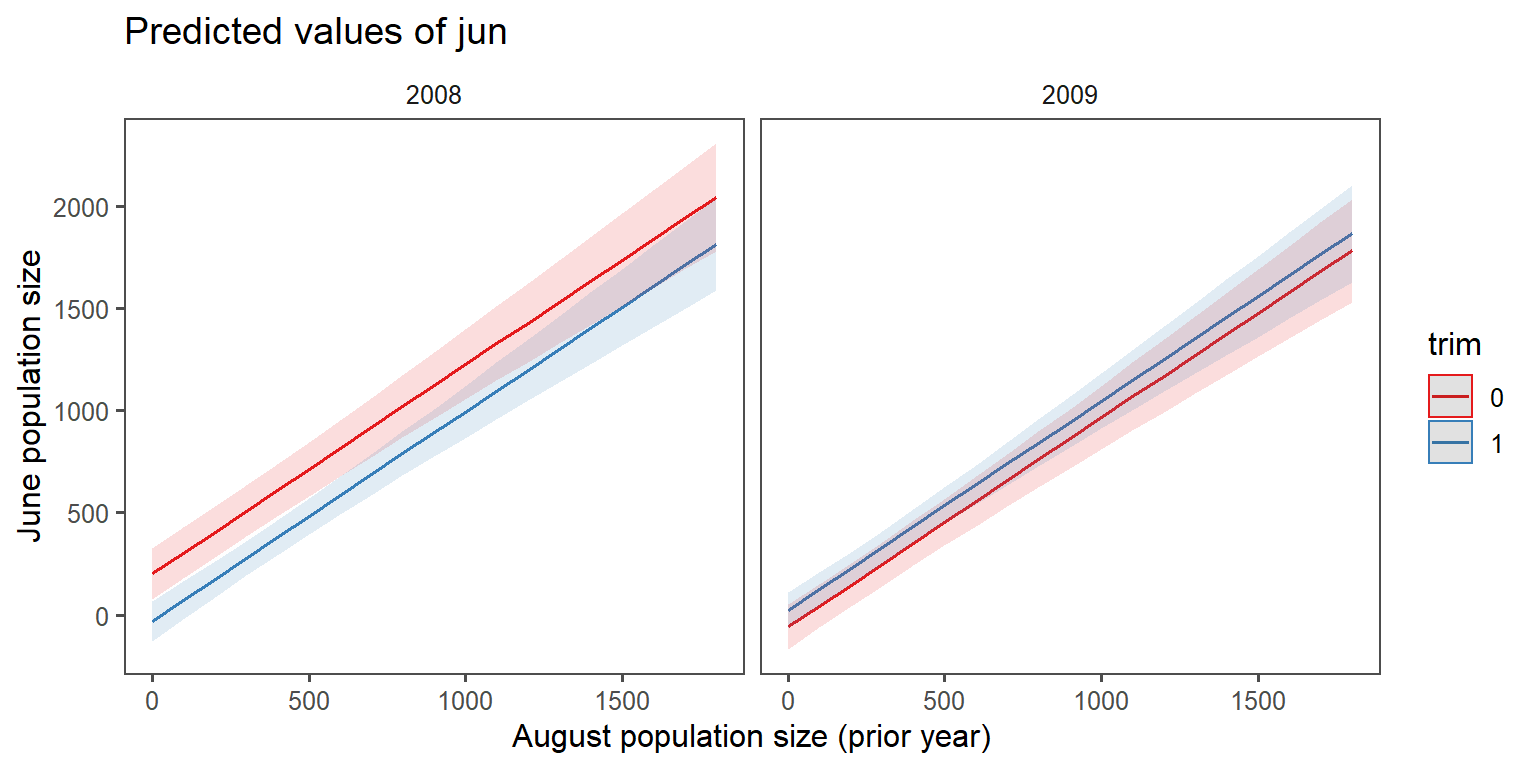
\includegraphics{C:\Users\phyll\RPROJE~1\POSTEL~1\docs\INDEX_~1/figure-latex/pop-plot-1} \hfill{}

\textbackslash caption\{Modeled recruitment and effects with 95\% confidence bands (from the mixed model).\}(\#fig:pop-plot)
\textbackslash end\{figure\}

\begin{quote}
In 2007, frond harvesting reduced frond sizes at the end of the growth season and dramatically reduced spore production, especially when done in the summer instead of in spring (Thompson et al 2010). There is strong evidence that the reduced reproductive output in 2007, due to frond harvesting, yielded lower juvenile recruitment (smaller populations) in 2008 .
\end{quote}

\newpage

\hypertarget{reduction-of-postelsia-population-sizes-during-the-growth-season}{%
\section{\texorpdfstring{Reduction of \emph{Postelsia} population sizes during the growth season}{Reduction of Postelsia population sizes during the growth season}}\label{reduction-of-postelsia-population-sizes-during-the-growth-season}}

\begin{quote}
The size of \emph{Postelsia} populations consistently declined over the summer months of three years (2007, 2008, 2009) by about 50\% with no difference among years or with respect to frond harvesting. As shown in Figure @ref(fig:popchangejun-aug) below if a population of \emph{Postelsia} has 1000 plants in June, it will have only 573 plants by August (1000 x 0.53 + 43 = 573).
\end{quote}

\begin{figure}

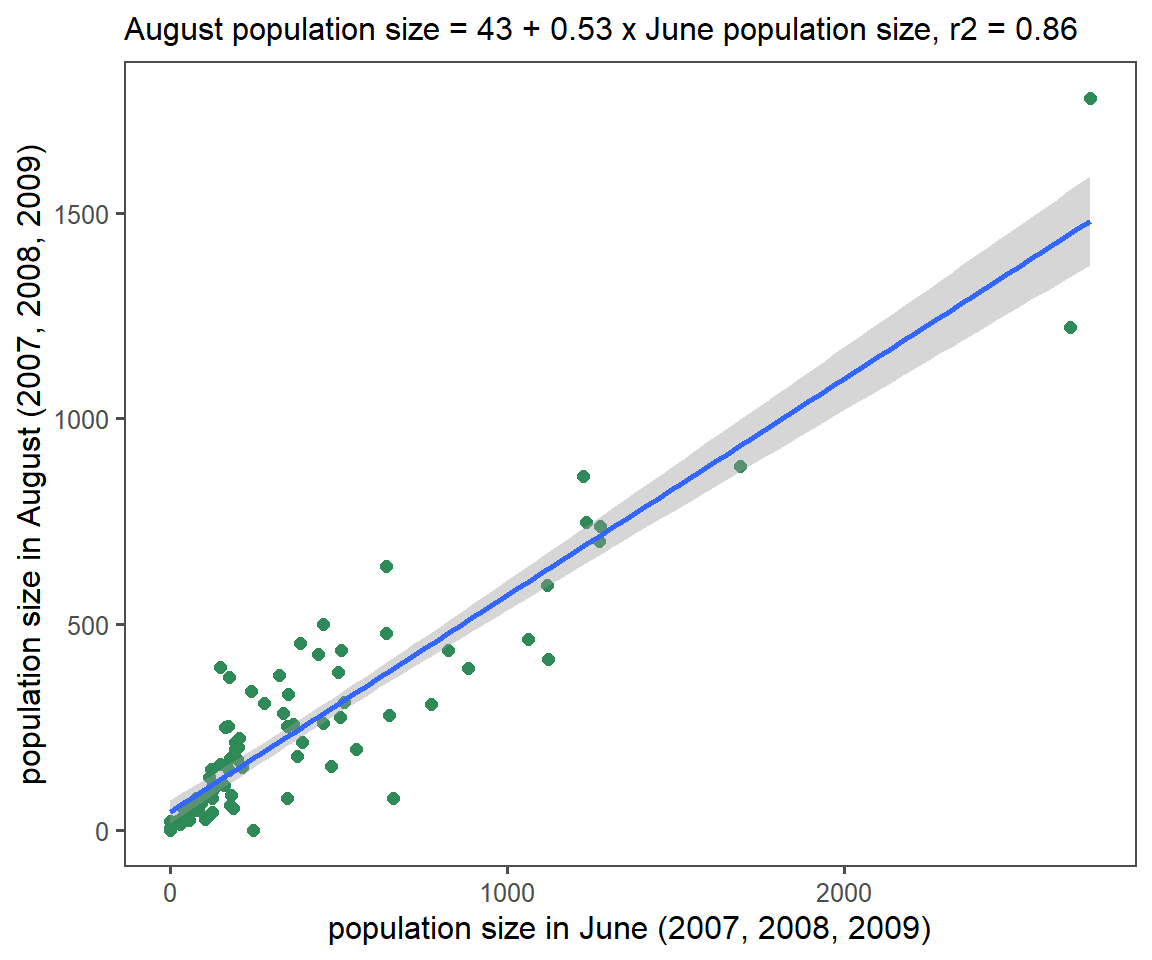
\includegraphics{C:\Users\phyll\RPROJE~1\POSTEL~1\docs\INDEX_~1/figure-latex/popchangejun-aug-1} \hfill{}

\caption{Decline in population size between June and August.}(\#fig:popchangejun-aug)
\end{figure}

This is likely a natural thinning process driven by the dislodgement of larger or poorly-attached thalli (``plants'') by waves. Crowding and resulting etiolated growth or intra-specific competition for light may also contribute. These dislodged plants fuel wrack-based food webs on sandy beaches, may help colonize other locations by transporting reproductive individuals to new locations, or may even be transported to deeper waters, contributing to carbon sequestration (Krause-Jensen \& Duarte 2016, Ortega et al.~2019). By August, most populations are have reproductive adults and will likely contribute to the next generation.

\newpage

\hypertarget{effects-of-tidal-height-interannual-environmental-variation-and-frond-trimming-on-individuals}{%
\section{Effects of tidal height, interannual environmental variation, and frond trimming on individuals}\label{effects-of-tidal-height-interannual-environmental-variation-and-frond-trimming-on-individuals}}

We suspect that variation in environmental conditions between years affects whether frond harvesting affects population dynamics. Differences in water temperature, nutrients, air temperature, tidal elevation, etc. may affect growth, survivorship, or the reproductive potential of individual plants at different times of the year. Different environmental factors may impact the two different life history stages at different times of year as well. We know very little about how field conditions affect the microscopic gametophyte stages.

\hypertarget{biomass}{%
\subsection{Biomass}\label{biomass}}

The diameter of the base of the stipe of an individual \emph{Postelsia} thallus or ``plant'' is an excellent predictor of the dry weight or biomass of the plant (Figure @ref(fig:diam-dw-fig)). Measurements of stipe diameter in the field are a convenient and non-destructive way to estimate \emph{Postelsia} growth or production without sacrificing plants. We collected 22 plants to assess the relationship between biomass.

\begin{figure}

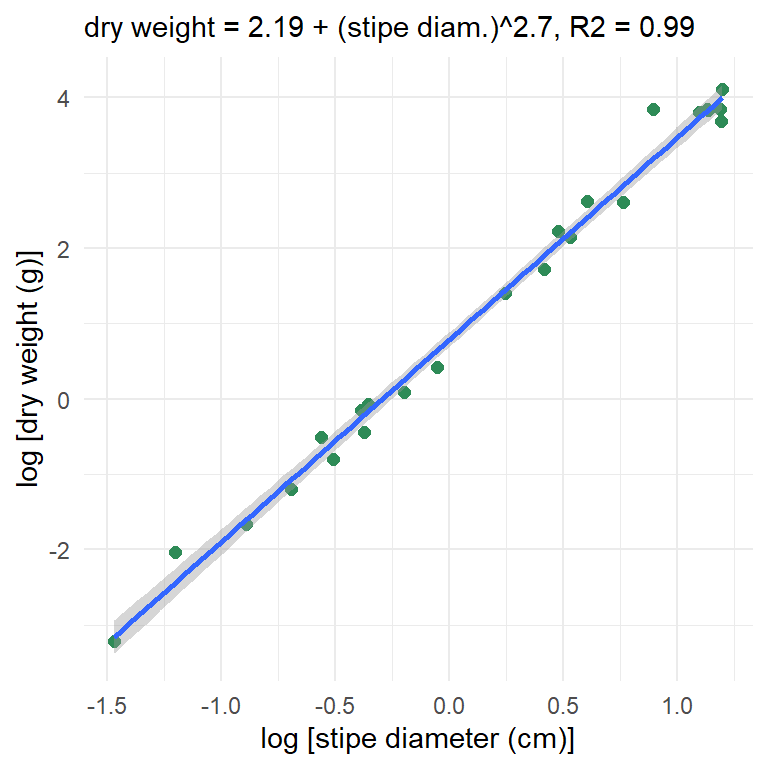
\includegraphics{C:\Users\phyll\RPROJE~1\POSTEL~1\docs\INDEX_~1/figure-latex/diam-dw-fig-1} \hfill{}

\caption{ Relationship between *Postelsia* biomass and stipe diameter}(\#fig:diam-dw-fig)
\end{figure}

\begin{quote}
Using stipe diameter as a proxy for biomass, we found that plants from populations higher in the intertidal zone produced less biomass than those lower in the intertidal zone (Figure @ref(fig:plot-bm-model-fit, Table 6.1), consistent with prior research (Nielsen et al.~2006).
\end{quote}

This is most likely due to longer emersion times in the upper intertidal zone that reduce access to nutrients in the water, exposes the plants to atmospheric conditions for longer periods of time, resulting in additional desiccation and heat stress. \emph{Postelsia} growing higher on the shore have lower nitrogen content and higher C:N ratios than those lower in the shore (Nielsen et al.~2006).

\begin{quote}
In addition, variation in annual conditions affected stipe diameter, the height of plants, and their reproductive status at the end of the annual growth season. Plants in 2009 produced less biomass, were shorter, and had a smaller proportion of individuals with visible sori (where spores are formed) (Figures @ref(fig:plot-bm-model-fit), @ref(fig:plot-h-model-fit), and @ref(fig:plot-pr-model-fit)).
\end{quote}

\begin{quote}
Those that had their fronds harvested had less biomass in August, but the statistical evidence for this was moderate (Figure @ref(fig:pop-plot), Table 6.1). They were also shorter and had a smaller proportion of individuals with visible sori (Figures @ref(fig:plot-h-model-fit) and @ref(fig:plot-pr-model-fit)). Over the range of tidal heights examined in this study, we did not see variation in plant height or reproductive status with tidal height (Tables 6.2 and 6.3). However, this study was not set up to examine tidal height variation per se, so this is not an unexpected result for these metrics.
\end{quote}

\newpage

Table 6.1. Linear mixed model of \emph{Postelsia} stipe diameter, a proxy for biomass.

~

Stipe diameter

Predictors

Estimates

Conf. Int (95\%)

p-Value

Intercept

30.27

26.91~--~33.64

\textless0.001

Harvested

-1.82

-3.75~--~0.10

0.064

2008

-1.33

-3.57~--~0.91

0.244

2009

-3.78

-6.06~--~-1.50

0.001

Tidal height

-1.01

-1.66~--~-0.36

0.002

Random Effects

σ2

19.62

τ00 site\_code

0.83

ICC

0.04

N site\_code

4

Observations

88

Marginal R2 / Conditional R2

0.218 / 0.249

The response variable is the stipe diameter of adult \emph{Postelsia} plants in August, the end of the growth season. The explanatory variables are tidal height of the population (th), and indicator variable for the frond harvest treatment (trim\_all, where 1 = fronds were harvested, 0 = fronds were left intact), the year (yr\_f, where year is 2007, 2008 or 2009). Sites were included as a random factor to account for the stratified randomization of trimming treatments within sites and to account for any differences in environmental conditions among sites that might affect individual performance.

\textbackslash begin\{figure\}

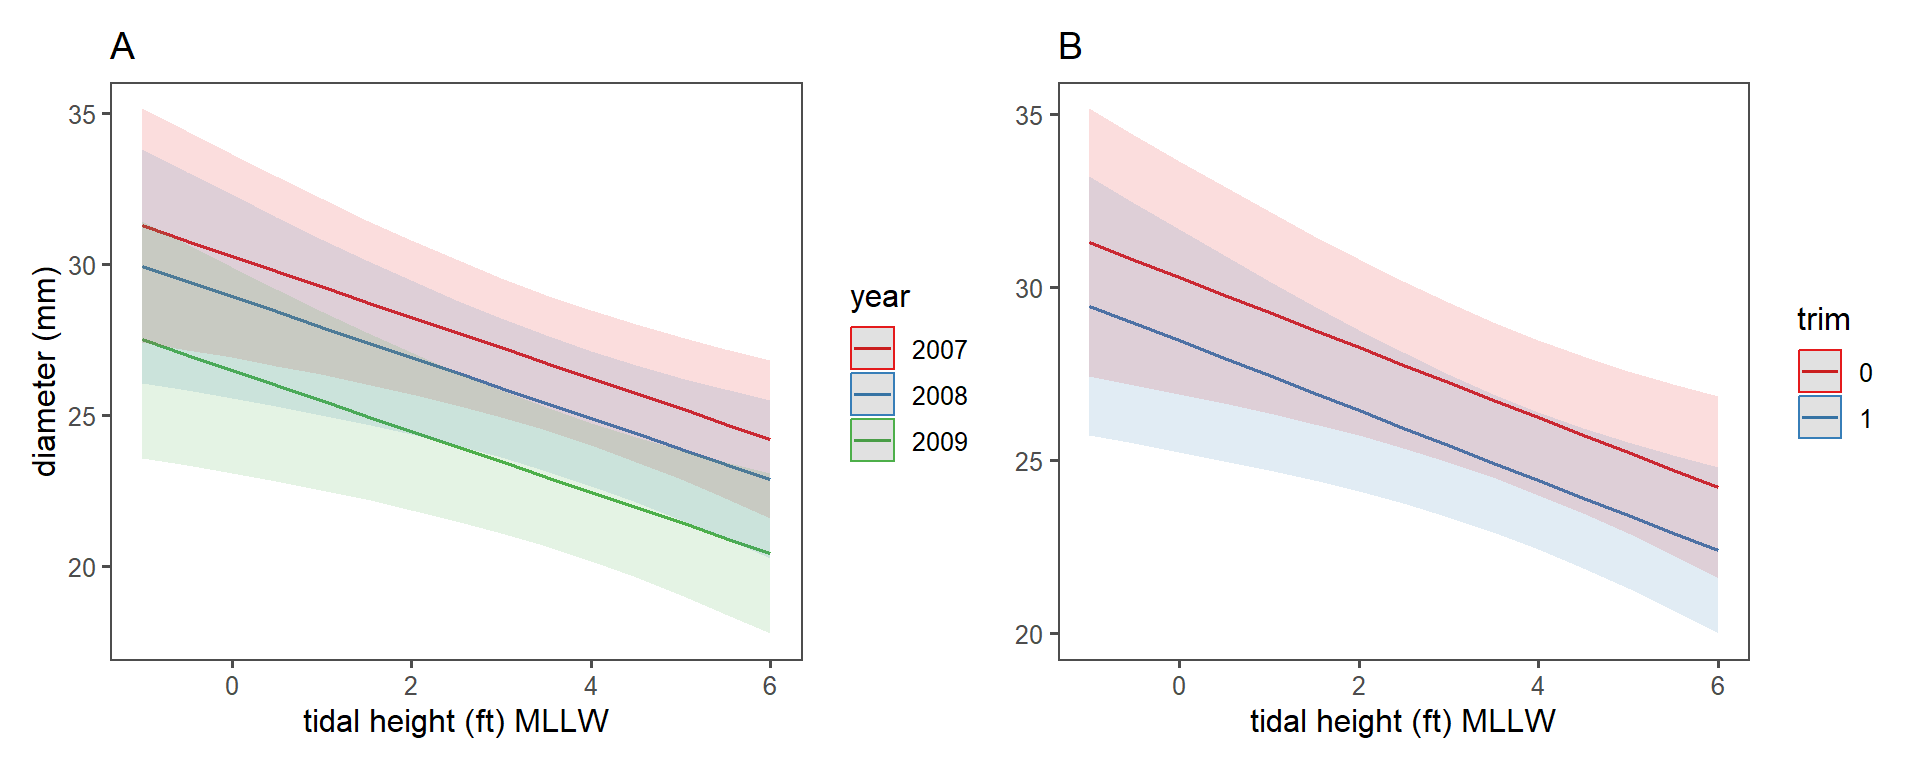
\includegraphics{C:\Users\phyll\RPROJE~1\POSTEL~1\docs\INDEX_~1/figure-latex/plot-bm-model-fit-1} \hfill{}

\textbackslash caption\{Modeled stipe diameter and effects with 95\% confidence bands (from the mixed model). A) effect of year and B) effect of frond harvesting (where=1 indicates trimmed, and 0 = not trimmed)\}(\#fig:plot-bm-model-fit)
\textbackslash end\{figure\}

\newpage

\hypertarget{size-height}{%
\subsection{Size (height)}\label{size-height}}

Table 6.2. Linear mixed model of \emph{Postelsia} size (height).

~

Stipe height

Predictors

Estimates

Conf. Int (95\%)

p-Value

Intercept

37.58

32.01~--~43.15

\textless0.001

Harvested

-3.79

-6.58~--~-1.01

0.008

2008

-2.17

-5.40~--~1.07

0.189

2009

-7.06

-10.36~--~-3.76

\textless0.001

Tidal height

-0.65

-1.66~--~0.35

0.203

Random Effects

σ2

40.90

τ00 site\_code

7.48

ICC

0.15

N site\_code

4

Observations

88

Marginal R2 / Conditional R2

0.214 / 0.336

The response variable is the stipe height of adult \emph{Postelsia} plants in August, the end of the growth season. The explanatory variables are as in Table. 6.1.

\textbackslash begin\{figure\}

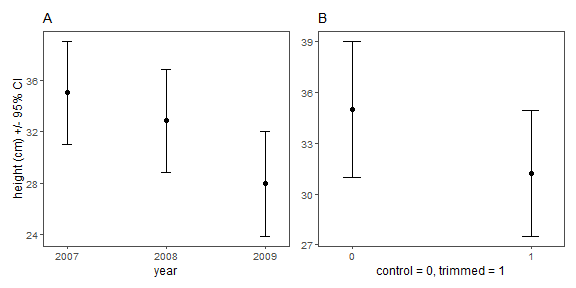
\includegraphics{C:\Users\phyll\RPROJE~1\POSTEL~1\docs\INDEX_~1/figure-latex/plot-h-model-fit-1} \hfill{}

\textbackslash caption\{Modeled stipe height and effects of year and frond harvesting with 95\% confidence intervals (from the mixed model). A) effect of year and B) effect of frond harvesting (where=1 indicates trimmed, and 0 = not trimmed)\}(\#fig:plot-h-model-fit)
\textbackslash end\{figure\}
\newpage

\#\#Reproductive status

Table 6.3. Linear mixed model of \emph{Postelsia} reproductive status.

~

Proportion reproductive

Predictors

Odds Ratios

Conf. Int (95\%)

p-Value

Intercept

1.52

0.34~--~6.90

0.586

Harvested

0.36

0.14~--~0.92

0.032

2008

3.12

1.04~--~9.38

0.043

2009

0.69

0.22~--~2.17

0.522

Tidal height

0.89

0.66~--~1.20

0.444

Random Effects

σ2

3.29

τ00 site\_code

0.00

N site\_code

4

Observations

0

Marginal R2 / Conditional R2

0.000 / NaN

The response variable is the proportion of adult \emph{Postelsia} plants that had visible sori in August. The explanatory variables are as in Table. 6.1.

\textbackslash begin\{figure\}

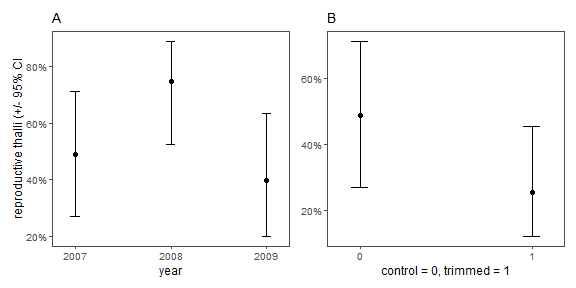
\includegraphics{C:\Users\phyll\RPROJE~1\POSTEL~1\docs\INDEX_~1/figure-latex/plot-pr-model-fit-1} \hfill{}

\textbackslash caption\{Modeled reproductive status and effects of year and frond harvesting with 95\% confidence intervals (from the mixed model). A) effect of year and B) effect of frond harvesting (where=1 indicates trimmed, and 0 = not trimmed)\}(\#fig:plot-pr-model-fit)
\textbackslash end\{figure\}
\newpage

\hypertarget{impact-of-frond-harvesting-on-frond-growth-and-reproductive-output}{%
\section{Impact of frond harvesting on frond growth and reproductive output}\label{impact-of-frond-harvesting-on-frond-growth-and-reproductive-output}}

Previously published results (Thompson et al., 2010) found that the area of fronds are smaller and reproductive output is lower overall in the southernmost site they studied (Piedras Blancas). The fronds of unharvested \emph{Postelsia} were largest between June and July, and reached their maximum size at the southernmost site about a month earlier. Piedras Blancas was near the biogeographic range limit for the species at the time of the study and differences in environmental conditions between the regions may be contributing to these differences in ecological performance.

Frond harvesting reduced frond area overall at the end of the growth season, regardless of when trimming was done or how often it was done. Fronds cut in the spring were able to regrow, while those cut in late July, after the onset of reproduction, did not (Thompson et al., 2010).

Reproductive output of viable spores for most individuals did not begin until late July at both sites, just after the fronds obtained their maximum size. It was greatest between September and October overall. At Point Cabrillo, the northern California site, sea palms trimmed in late July for either the first or second time had dramatically reduced reproductive output in September, compared to those not harvested at all. At the southern site, observations made in October were qualitatively similar.

\newpage

\hypertarget{interannual-variation-in-monthly-nitrogen-availablity-from-coastal-upwelling}{%
\section{Interannual variation in monthly nitrogen availablity from coastal upwelling}\label{interannual-variation-in-monthly-nitrogen-availablity-from-coastal-upwelling}}

One possible contributing factor to the variations among years in individual biomass, size, and reproductive status is the availability of nitrogen delivered through coastal upwelling during the growth season. The annual frequency, duration, and seasonal timing of coastal upwelling, which delivers cold, nutrient-rich waters to coastal ecosystems, are important drivers of marine primary productivity in northern California marine ecosystems.

In 2009 nitrogen supply as indexed by BEUTI (Biologically Effective Upwelling Transport Index) \href{https://agupubs.onlinelibrary.wiley.com/doi/full/10.1029/2018JC014187}{(Jacox et al.~2018)} was reduced during June and July compared to 2007 and 2008 (Figure @ref(fig:barplots). This may have had a negative influence on growth and production of \emph{Postelsia} in 2009. Additional explanatory information on the BEUTI index is available \href{https://mjacox.com/upwelling-indices/}{here}.

\begin{figure}

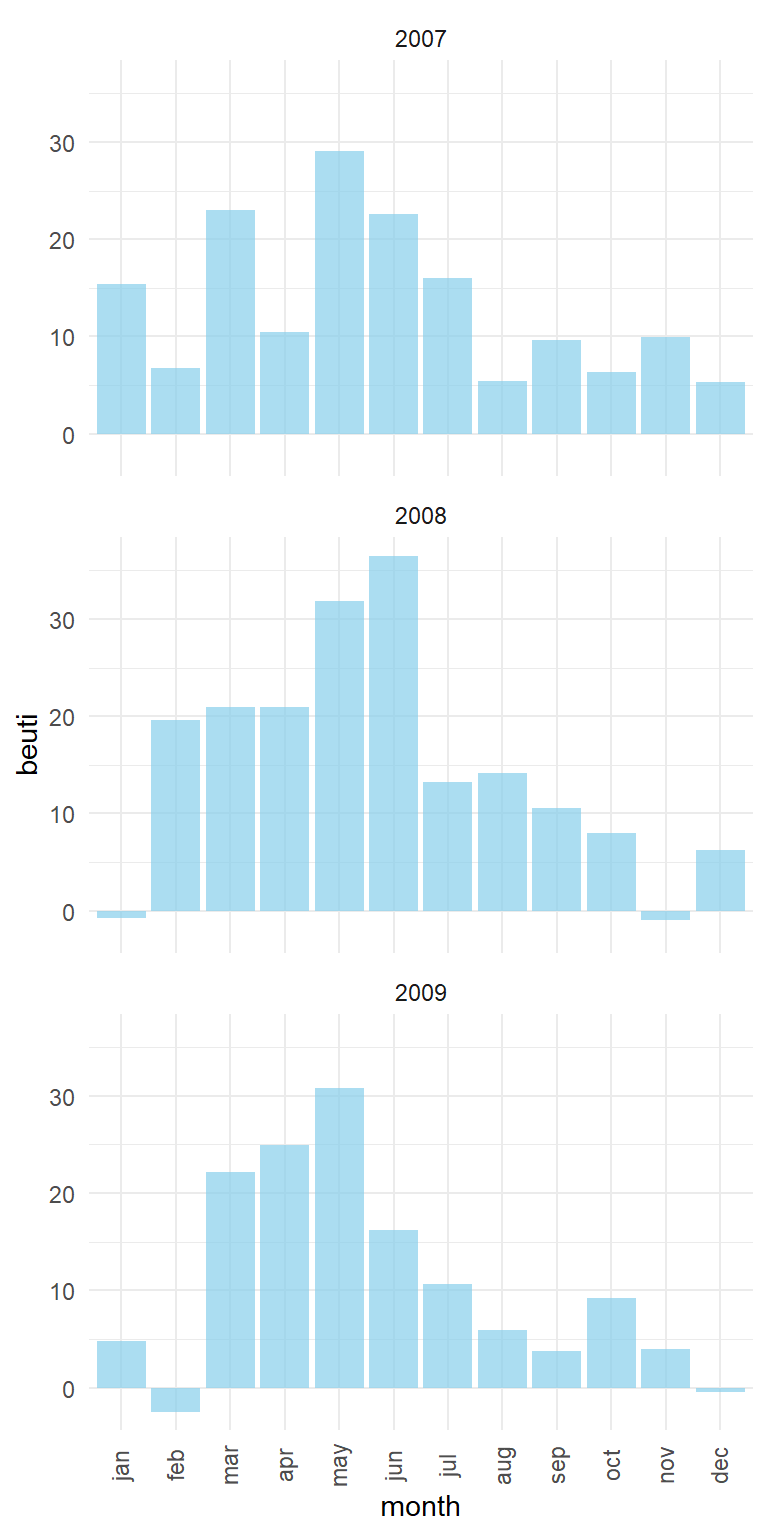
\includegraphics{C:\Users\phyll\RPROJE~1\POSTEL~1\docs\INDEX_~1/figure-latex/barplots-1} \hfill{}

\caption{Biologically Effective Upwelling Transport Index (BEUTI) for 2007, 2008, and 2009.}(\#fig:barplots)
\end{figure}

Warmer waters such as during recent marine heat waves \href{https://www.nature.com/articles/s42003-021-01827-6}{(McPherson et al.~2021)} may also have a negative impact on \emph{Postelsia}. A study of temperature tolerances of seaweeds (Lüning \& Freshwater 1988) determined that \emph{Postelsia} do not survive in waters above 15 °C. Sub-lethal effects of warmer waters may occur at somewhat lower temperatures.

\newpage

\hypertarget{implications-for-stewardship}{%
\section{Implications for stewardship}\label{implications-for-stewardship}}

If the growth or reproductive output of \emph{Postelsia} are affected by multiple impacts or stressors over the growth season, then population sizes may be reduced in subsequent years. If the frequency of ``bad years'' increases or bad conditions persist for longer during the growth season, especially in combination with other factors that reduce vital rates, then larger scale and longer term losses might be anticipated.

Thompson et al.~(2010) discussed a range of management approaches that would apply precautionary principles to protect \emph{Postelsia} populations from the risk of unanticipated growth in commercial seaweed harvesting. If commercial sea palm harvesting is allowed, they recommended that the non-lethal frond trimming method be required for as a condition of the commercial harvest license. They also recommended that fronds should only be harvested once a year. This probably requires spatial management since multiple commercial harvesters may collect from the same intertidal areas. Lastly, since the fronds don't readily grow back after sori develop, harvesting should be limited to spring.

Additionally, recent research on \emph{Postelsia} metapopulation dynamics by Paine et al.~(2017) shows that local populations can and do go extinct but are usually repopulated by zoospores dispersing from nearby populations (Figure @ref(fig:post-extinct)). However, they also showed that populations can remain locally extinct for decades to centuries if there are no nearby populations (within 20-30 meters) to supply spores (Paine et al.~2017).

\begin{figure}

\includegraphics[width=0.5\linewidth]{https://esajournals.onlinelibrary.wiley.com/cms/asset/744c48fe-044a-4fbc-b776-16f5c2144824/ecy1798-fig-0005-m} \hfill{}

\caption{Annual probabilities of *Postelsia* (A) colonization and (B) extinction in habitat patches as a function of distance from the nearest occupied site. [Paine et al. (2017)](https://esajournals.onlinelibrary.wiley.com/doi/10.1002/ecy.1798).}(\#fig:post-extinct)
\end{figure}

This has serious implications for the recovery of populations that have gone locally extinct, especially if the declines are widespread and there is no nearby source of spores to repopulate the location. WHile rafting of fertile plants from other sites does occur, it is rare over ecological time scales (Paine et al.~2017).

It is possible to (re-)establish new populations of \emph{Postelsia} by attaching fertile plants from another location to the rocks if the environmental conditions are suitable (as was done in experiments by Paine et al.~1973, Blanchette et al.~1996 in WA and OR, respectively). However, the methods are labor intensive and involve working on some of the most wave-exposed rocky shores in the region.

\begin{quote}
A precautionary approach to the stewardship of \emph{Postelsia palmaeformis} is warranted.
\end{quote}

\newpage

\hypertarget{methods-summary-for-unpublished-data-and-new-analyses}{%
\section{Methods summary for unpublished data and new analyses}\label{methods-summary-for-unpublished-data-and-new-analyses}}

Individual populations were monitored at four different sites in Sonoma and Marin counties in California for three years. Populations were selected based on ability to safely access them and make measurements. As a consequence, the most wave exposed populations, and those lowest in the intertidal zone, were not well represented in this study. We also did not target populations distributed at the upper most fringe of the species intertidal distribution. WIthin each site, populations were randomly assigned as either controls or to have their fronds trimmed in each of three years (2007, 2008, 2009). Ten visually representative plants from each population were haphazardly selected and their stipe diameters were measured at the base of the stipe immediately above the haptera of the holdfast. Tidal height of each population was measured using a stadia rod and level scope with reference to a local still water level at a known time and scaled using local tidal height predictions.

We modeled juvenile recruitment (June population size) using linear mixed models with year (to represent inter annual variation in environmental conditions), the adult population size in August of the prior year, and the frond harvest treatment as fixed factors. We included site as a random factor to account for the randomization of trimming treatments within sites and the known metapopulation dynamics of populations within a local site. We did not include tidal height as a factor as it is inherently represented by the August population size. To assess individual plant metrics within populations (stipe diameter and height, and proportion of plants that were reproductive with visible sori) we modeled the frond harvest treatment, tidal height, and year as fixed factors and site as a random factor. We checked model fit by visual inspection of residual plots. Interaction terms were initially included, but were dropped if they did not improve model fit as our questions of interest involved the main effects.

\hypertarget{references}{%
\section{References}\label{references}}

Please see this \href{https://www.zotero.org/groups/4289135/postelsia_palmaeformis/library}{Zotero library}.

\end{document}
